% 图 81.5 —— **结构化重画**（2026-09-25，替换掉 `checks/emit_hand.py` 的逐段拟合稿）
%%
% 结构：4 个两两外切的圆（半径两档）+ 3 个切点实心点 + 6 支切向箭头 + 14 个标签
%%
% 旧版是**描摹**：把每一段笔画单独拟合后发出来，连「箭头头」都被当成"一条很粗的短线"描
%   （图 81.5 上一度出现 `\draw[line width=7.0pt] (586,277)--(586,270);` 这种 7px 长的疙瘩），
%   渲染出来是黑疙瘩而不是箭头。本版改成**看懂结构后用 TikZ 画**。
%%
% 做法、约定、已踩过的坑 → `＜工作区＞\checks\redraw\README_重画流程.md`
% 本图圆/椭圆的中心与半径、标签的文字与位置，沿用 probe 的脚手架（那部分它是对的）。
%%
% ⚠ 本图 tikzpicture 是 y=-1pt（**y 翻转**）⇒ `arc` 的角向"递减"才是屏幕逆时针；
%   同一根线上的多段弧必须同向。改完务必拿原书并排、放大核箭头朝向。
%%
\documentclass[12pt]{standalone}
\usepackage{fontspec}
\setsansfont{Arial}
\newfontfamily\mfallback{DejaVu Sans}
\usepackage{tikz}
\usetikzlibrary{arrows.meta}
\begin{document}
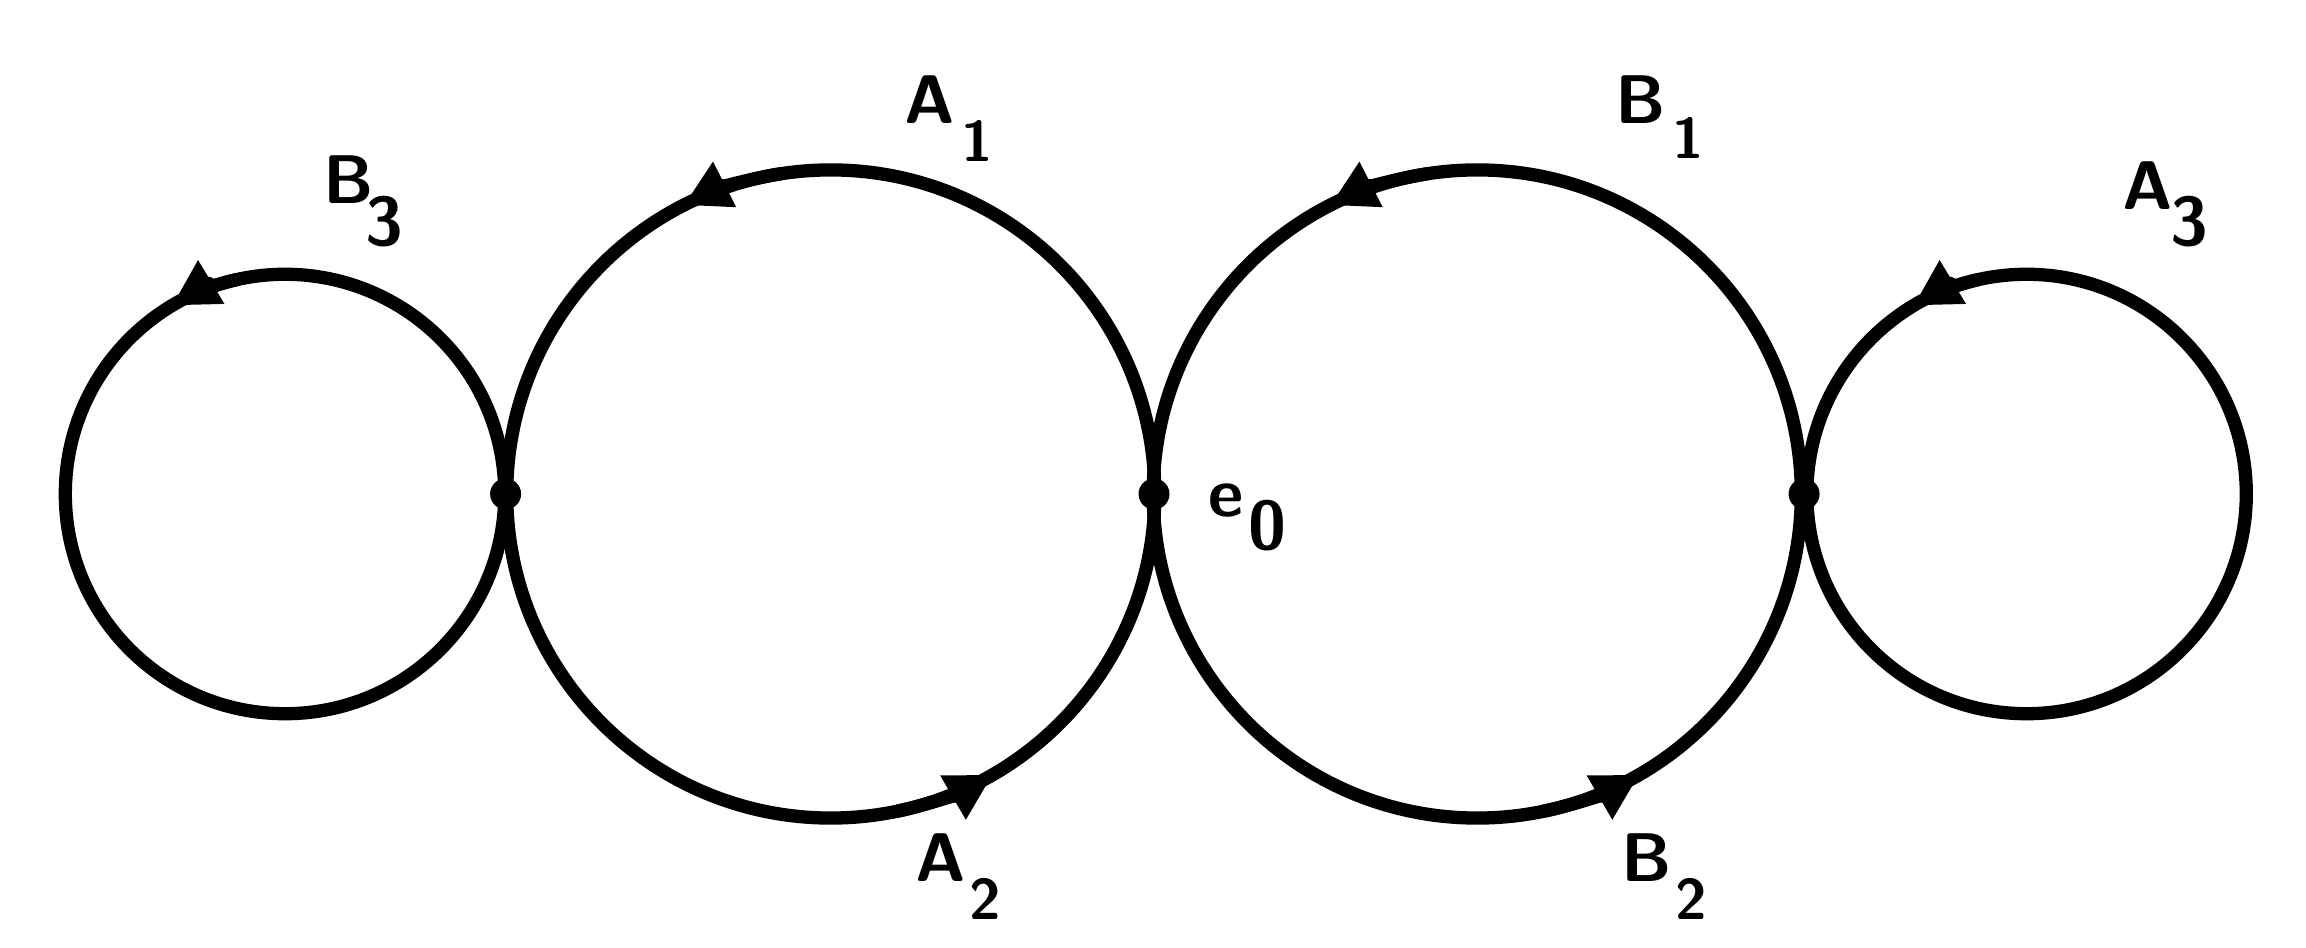
\begin{tikzpicture}[x=1pt, y=-1pt, line width=4.8pt, line cap=round, line join=round]
  % ---- 箭头（2026-09-25）-----------------------------------------------------
  % 样式与全库一致：标准 `-{Triangle[width=..,length=..]}`，不自创图元。
  % ⚠ 关键：**箭头弧要短**。把圆画成 circle、箭头画成一条**长**弧时，长弧在
  %   `y=-1pt`（y 翻转）下会累积约 0.75pt 的径向漂移，两条笔画不重合、并集外扩
  %   ⇒ "箭头后的部分很粗"。实测（r=79.4）：
  %       圆            θ=258° 外缘 +2.99  宽 5.22
  %       长弧 340→239            +3.74      5.55   ✗
  %       短弧 256→239            +2.63      4.44   ✓ 与圆重合
  %   所以箭头只挂 ~18°（≈头长）的短弧；外溢的部分盖在圆上，看不见。
  \def\arr{-{Triangle[width=17.2pt,length=16.6pt]}}
  \def\arrowarc#1#2#3#4{%
    \draw[\arr] (#1,#2) ++(#4+18:#3) arc[start angle=#4+18, end angle=#4, radius=#3];%
  }
  % 2026-09-25 修：头**偏小**。原书 600dpi 圆弧径向剖面（带心自标定）：原书头宽 17.2 pt，

  % ── 四个相切的圆：一行 \foreach ──（半径只有两档 79.4 / 117.1，圆心同高）
  \foreach \x/\r in {93.0/79.4, 290.2/117.1, 523.8/117.1, 722.3/79.4}
    \draw (\x,168.5) circle (\r);

  % ── 三个切点上的实心点 ──
  \foreach \x in {172.7, 407.0, 641.9} \fill (\x,168.5) circle (5.6);

  % ── 圆上的切向箭头：arc + Triangle，箭头头白送 ──
  \arrowarc{93.0}{168.5}{79.4}{239}
  \arrowarc{722.3}{168.5}{79.4}{239}
  %% ⚠ 本图 tikzpicture 是 y=-1pt（y 翻转）⇒ **角向递减 = 屏幕上的逆时针**。
  %%    两条弧必须**同向**（都递减）；写成一递增一递减会把下弧的头甩到 7 点钟、方向也反。
  \foreach \cx in {290.2, 523.8} {
    \arrowarc{\cx}{168.5}{117.1}{243}
    \arrowarc{\cx}{168.5}{117.1}{60}
  }
  % ⚠ 这里**没有弧** —— 2026-09-25 我曾在 A₁/B₁ 切点处凭空加过一条"e₀ 弧"，
  %   放大原图（8×，带坐标网格）后确认：切点处只有一个实心点，右边是 `e` `0` 两个字母。
  %   **是我把字母 e 误看成了弧。** 已删。

  % ── 标签 ──
  \node[anchor=center,inner sep=0pt,font=\fontsize{29.6}{37.0}\selectfont] at (326,26) {\textsf{\textbf{\textit{A}}}};
  \node[anchor=center,inner sep=0pt,font=\fontsize{22.2}{27.8}\selectfont] at (343,41) {\textsf{\textbf{1}}};
  \node[anchor=center,inner sep=0pt,font=\fontsize{29.6}{37.0}\selectfont] at (583,26) {\textsf{\textbf{\textit{B}}}};
  \node[anchor=center,inner sep=0pt,font=\fontsize{22.2}{27.8}\selectfont] at (600,40) {\textsf{\textbf{1}}};
  \node[anchor=center,inner sep=0pt,font=\fontsize{30.3}{37.9}\selectfont] at (116,55) {\textsf{\textbf{\textit{B}}}};
  \node[anchor=center,inner sep=0pt,font=\fontsize{23.0}{28.7}\selectfont] at (129,70) {\textsf{\textbf{3}}};
  \node[anchor=center,inner sep=0pt,font=\fontsize{29.6}{37.0}\selectfont] at (766,57) {\textsf{\textbf{\textit{A}}}};
  \node[anchor=center,inner sep=0pt,font=\fontsize{23.0}{28.7}\selectfont] at (781,70) {\textsf{\textbf{3}}};
  \node[anchor=center,inner sep=0pt,font=\fontsize{32.4}{40.5}\selectfont] at (433,171) {\textsf{\textbf{\textit{e}}}};
  \node[anchor=center,inner sep=0pt,font=\fontsize{24.9}{31.1}\selectfont] at (448,180) {\textsf{\textbf{0}}};
  \node[anchor=center,inner sep=0pt,font=\fontsize{29.6}{37.0}\selectfont] at (330,300) {\textsf{\textbf{\textit{A}}}};
  \node[anchor=center,inner sep=0pt,font=\fontsize{22.2}{27.8}\selectfont] at (346,315) {\textsf{\textbf{2}}};
  \node[anchor=center,inner sep=0pt,font=\fontsize{29.6}{37.0}\selectfont] at (585,300) {\textsf{\textbf{\textit{B}}}};
  \node[anchor=center,inner sep=0pt,font=\fontsize{22.2}{27.8}\selectfont] at (601,315) {\textsf{\textbf{2}}};

  \path[use as bounding box] (0,0) rectangle (813,318);
\end{tikzpicture}
\end{document}
